\subsubsection{UC25 - Visualizzazione singolo messaggio}\label{UC25}
\paragraph*{Descrizione}
L'Utente visualizza un messaggio nella chat. Questo può essere un messaggio di richiesta in linguaggio naturale o un messaggio di risposta contenente il \glossario{prompt}. 

\paragraph*{Attori principali}
Utente

\paragraph*{Precondizioni}
\begin{itemize}
  \item Dev'essere presente almeno un messaggio nella chat.
\end{itemize}

\paragraph*{Postcondizioni}
\begin{itemize}
  \item L'Utente visualizza correttamente il messaggio nella chat.
\end{itemize}

\paragraph*{Scenario principale}
\begin{enumerate}
  \item Nel sistema è presente almeno un messaggio della chat.
  \item L'Utente visualizza il messaggio.
\end{enumerate}

\paragraph*{Inclusioni}
\begin{itemize}
    \item Visualizzazione messaggio di richiesta (\hyperref[UC25point1]{UC25.1});
    \item Visualizzazione messaggio di risposta (\hyperref[UC25point2]{UC25.2});
\end{itemize}

\begin{figure}[H]
  \centering
  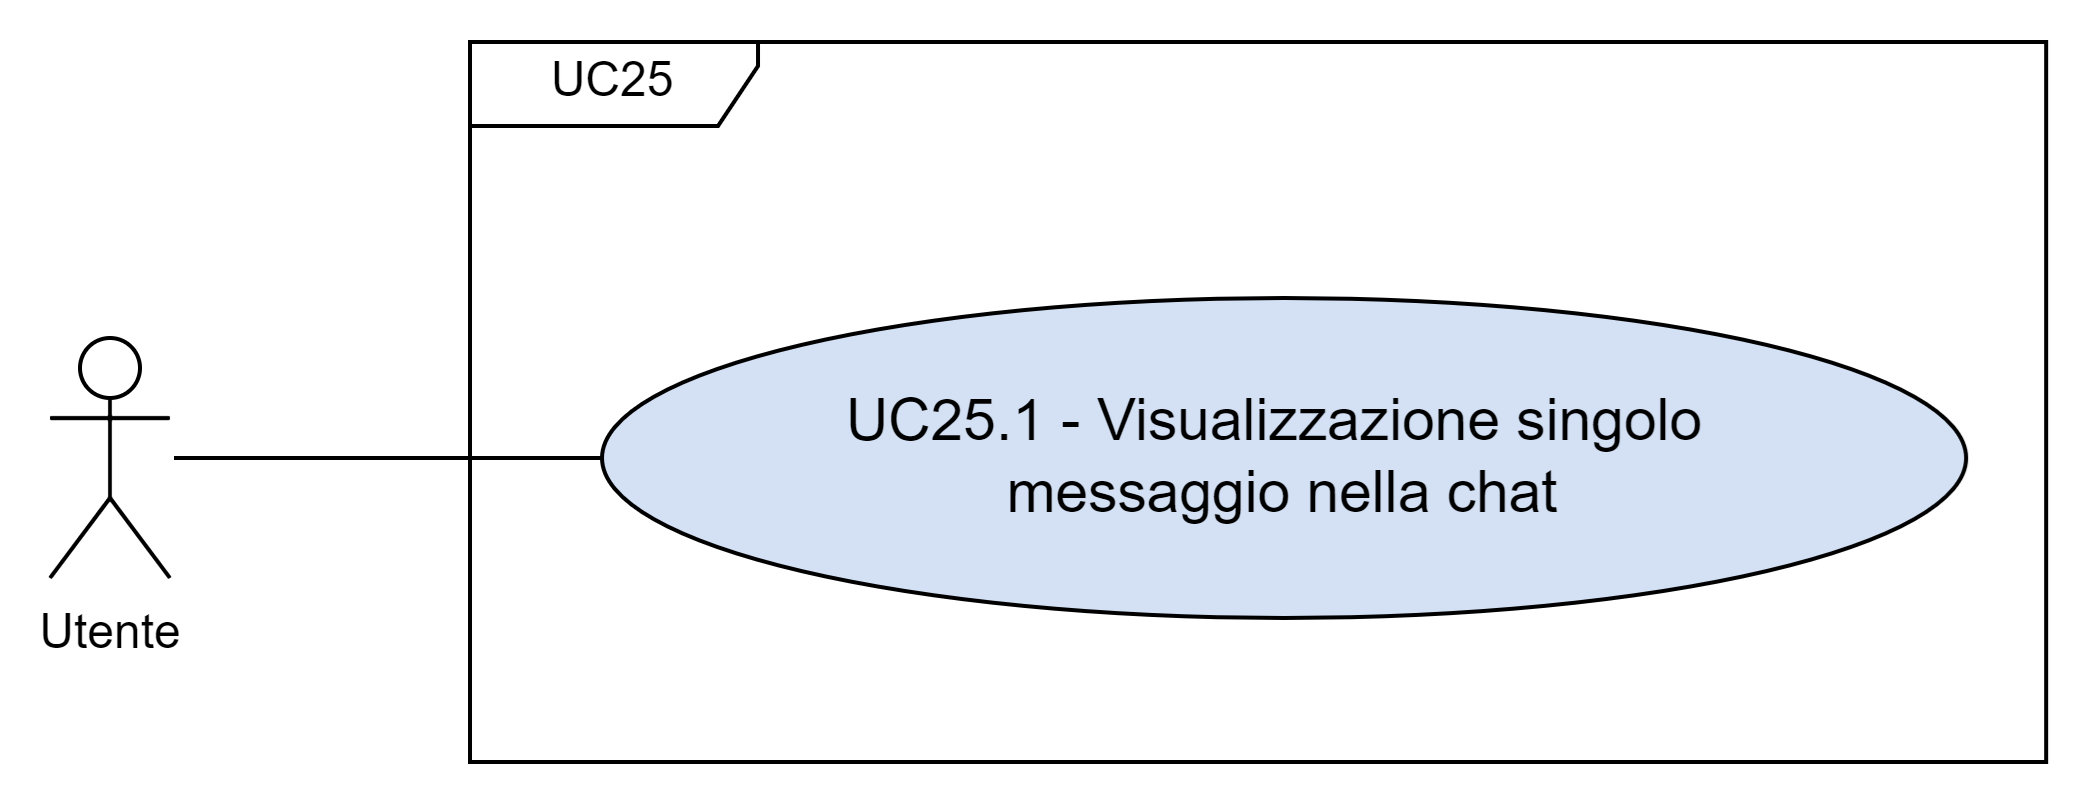
\includegraphics[width=0.90\textwidth]{assets/uc25.png}
  \caption{UC25 - Sottocasi d'uso}
\end{figure}

%%%%%%%%%%%%%%%%%%%%%%%%%%%%%%%%%%%%%%%%%%%

\subsubsection{UC25.1 - Visualizzazione messaggio di richiesta}\label{UC25point1}
\paragraph*{Descrizione}
L'Utente visualizza un messaggio con la sua richiesta in linguaggio naturale nella chat.

\paragraph*{Attori principali}
Utente

\paragraph*{Precondizioni}
\begin{itemize}
  \item È presente almeno un messaggio di richiesta in linguaggio naturale nella chat (\hyperref[UC3]{UC3}).
  \item L'Utente visualizza un messaggio nella chat.
\end{itemize}

\paragraph*{Postcondizioni}
\begin{itemize}
  \item Il messaggio visualizzato è un messaggio con una richiesta in linguaggio naturale.
\end{itemize}

\paragraph*{Scenario principale}
\begin{enumerate}
  \item Nel sistema è presente almeno un messaggio di richiesta in linguaggio naturale (\hyperref[UC3]{UC3}).
  \item L'Utente visualizza il messaggio di richiesta.
\end{enumerate}

%%%%%%%%%%%%%%%%%%%%%%%%%%%%%%%%%%%%%%%%%%%

\subsubsection{UC25.2 - Visualizzazione messaggio di risposta}\label{UC25point2}
\paragraph*{Descrizione}
L'Utente viualizza un messaggio di risposta, contenente il \glossario{prompt} generato da una richiesta in linguaggio naturale.

\paragraph*{Attori principali}
Utente

\paragraph*{Precondizioni}
\begin{itemize}
  \item È presente almeno un messaggio di risposta contenente un \glossario{prompt} (\hyperref[UC5]{UC5}).
  \item L'Utente visualizza un messaggio nella chat.
\end{itemize}

\paragraph*{Postcondizioni}
\begin{itemize}
  \item Il messaggio visualizzato è un messaggio con una riposta contenente un \glossario{prompt}.
\end{itemize}

\paragraph*{Scenario principale}
\begin{enumerate}
  \item Nel sistema è presente almeno un messaggio di risposta contenente un \glossario{prompt} (\hyperref[UC5]{UC5}).
  \item L'Utente visualizza il messaggio di riposta.
\end{enumerate}

